\documentclass[12pt]{article}
\usepackage[margin=0.5in]{geometry}
\usepackage{amsmath}
\usepackage{amssymb}
\usepackage{graphicx}
\usepackage{silence}
\WarningsOff[latex]
\usepackage{float}
\graphicspath{ {./pics/} }
\linespread{1.2}
\newcommand{\code}{\texttt}
\usepackage{csquotes}
\usepackage{algorithm}
\usepackage[noend]{algpseudocode}
\bibliographystyle{plain}
\usepackage[hyphens,spaces]{url}

\begin{document}
\subsection*{Q1.}
Since we use simple uniform hashing, the average number of elements that hash to the same array would be \(\alpha = \frac{n}{m}\), where \(n\) is the total number of elements in the hash table, and \(m\) is the number of slots.

\paragraph{(a).} Given that we use sorted arrays as the chaining components for the hash table:\\ On average, the time complexity for search would be \(O(1+\log(\alpha))\),  Here, \(O(1)\) is the time taken to compute \(h(k)\), and \(O(\log(\alpha))\) is the time to search for the key inside the array at slot \(h(k)\). We achieve logarithmic runtime as we could perform binary search on the sorted array, since arrays allow random access. However, if \(\alpha\) is very small, we would not have much benefit from the usual way of using linked list as the chaining component (runtime being \(O(1+\alpha)\)). But in the case that \(n \gg m\), then the runtime would improve.

\paragraph{(b).} Given that we need to run a merge sort every time we insert an element:\\
On average, the time complexity for insertion would be \(O(1+\alpha\log(\alpha))\), where \(O(1)\) is the time to compute \(h(k)\), and \(O(\alpha\log(\alpha))\) is the time to perform the merge sort on the array at slot \(h(k)\). If we do not keep track of the current number of elements in the array, then we also have an additional cost of \(O(\alpha)\) to search to the end for an empty spot, otherwise it would just take \(O(1)\) time to append. Or if we consider the cost to expand the array size, then we need \(O(\alpha)\) to copy the old array into the new one. Yet in the end, the insertion time would be worse than the original scheme of using linked lists, which only costs \(O(1)\) time to prepend the key.

\paragraph{(c).} Deletion with sorted arrays would remain the same as using linked lists, i.e. \(O(1 +\alpha)\). \(O(1)\) is the time to compute \(h(k)\), and \(O(\alpha)\) is the total cost for deletion. To delete, we first need to search for the key, so it takes \(O(\log(\alpha))\) to perform binary search, then remove the key by shifting all elements greater than the deleted key one slot to the left. In the worst case, the deleted key is the first element, so we need to shift all the remaining elements, which is \(O(\alpha)\). Since \(O(\log(\alpha)) \in O(\alpha)\), we have the overall cost for search-delete-shift as \(O(\alpha)\). With linked lists, deletion is also \(O(\alpha)\). We need to traverse the list to search for the previous element of the target, then change its pointer to the next element of the target (\(O(1)\)), and free memory for the target(\(O(1)\)). In the worst case, the target is the last element, so we require \(O(\alpha)\).

\subsection*{Q2.}
His claim is not correct for all situations. There is no guarantee that the leaves of a complete binary tree are on the same level. There could be missing right-most nodes on the last level. As illustrated in Figure 1, all internal nodes of a complete binary tree have two children, but the leaves here are not on the same level, meaning that if we color all nodes as black, the number of black nodes from root to a leaf is not the same for all paths. This violates the red black tree property:
\begin{displayquote}[][]
     For each node, all paths from this node to each of its leaves contain the same number of black nodes.
\end{displayquote}
Hence, it is not a red black tree in this case.
\begin{figure}[H]
     \centering
     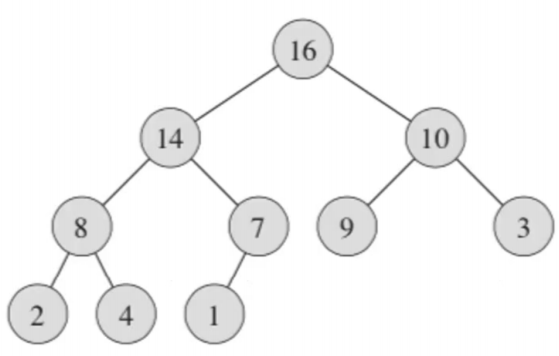
\includegraphics[scale =0.8]{q2a.png} 
     \caption{missing right-most nodes}
\end{figure}

\noindent However, if we have a perfect binary tree, which is a complete binary tree with all leaves on the same level (assuming leaves are nil), then it is valid red black tree:
     \begin{enumerate}
          \setlength \itemsep{0em} 
          \item the root is black
          \item leaves are black nils
          \item there is no consecutive red nodes along any path since there are no red nodes at all
          \item all paths from a node to its leaves contain the same number of black nodes.
     \end{enumerate}

\subsection*{Q3.}
An avl tree is a self balancing binary search tree that has the property that, for any node \(x\) in the tree, \(x\) has at most two children, and \(x.left.key \leq x.key \leq x.right.key\). Although for an avl tree, we might need rotation for insertion and deletion operations in order to maintain the balance factor, we still guarantee that the bst property holds. So the node with the minimum key is the left-most node in the tree. We could find it by traversing down the tree from the root, and always choosing the left subtree to traverse, until we find the left subtree to be nil, then the current node contains the minimum key. Similarly, the node with the maximum key is the right-most node in the tree. Beginning from the root, we always traverse the right subtree, until the right subtree is nil, then the current node contains the maximum key. 

\subsection*{Q4.}
\paragraph{(a).} Yes, we can solve it by dynamic programming.\\ 
Since the flat fee \(C\) remains constant for any sequence, we can just focus on the cost sum of flights in the sequence. In addition, since we need to find the cheapest sequence from any city-\(i\) to city-\(n\), the problem can be generalized to an all pairs shortest paths problem. We have to find cheapest sequence for all pairs, despite that the problem only asks for \((i,n)\). This is because the subsequence of a cheapest sequence is also a cheapest sequence by itself. We need to construct a cheapest-sequence tree (similar to shortest-path tree) for the ease of restoring sequences at the end. This algorithm will only need to be run quarterly when the prices of direct flights change. After that, we can simply answer customers' queries by looking up the cheapest-sequence tree. The underlying algorithm is Floyd-Warshall algorithm.

\pagebreak
\noindent\textbf{Sub-problems:} cheapest sequence to travel from city-\(i\) to city-\(j\) where \(i,j \in [1,n]\) using intermediate cities from the set \(\{1, \hdots, k\}\), and its length.\\
\textbf{Relation between sub-problems:}\\
 To build the cheapest sequence from city-\(i\) to city-\(j\) when the intermediate cities are taken from the set \(\{1, \hdots, k\}\), we notice that the sequence can either go through city-\(k\), or not. If it does, then the subsequences from city-\(i\) to city-\(k\), and from city-\(k\) to city-\(j\) would have intermediate cities taken from the set \(\{1, \hdots, k-1\}\). If it does not, then the sequence itself would have intermediate cities from \(\{1, \hdots, k-1\}\). Written as formulas,
\begin{itemize}
     \item On minimum cost:
     \begin{equation*}
          C_k (i,j) =
          \begin{cases}
               P(i, j) & k=0 \\
               \min (C_{k-1} (i, j), C_{k-1} (i, k) + C_{k-1} (k, j)) & k \geq 1
          \end{cases}
     \end{equation*}
     where \(C_k (i,j)\) denotes the minimum cost for travelling from city-\(i\) to city-\(j\) when the intermediate cities are from the set \(\{1, \hdots, k\}\)\\
     \(P(i,j)\) denotes the price of direct flight from city-\(i\) to city-\(j\). If there is no direct flight between two cities, the price would be \(\infty\).
     \item On cheapest sequence:\\
     For a pair of source and destination cities \((i, j)\), we store the next city of city-\(i\) on the cheapest sequence.
     \begin{equation*}
          N_k{(i,j)} =
          \begin{cases}
               j & \text{if } P(i, j) \neq \infty \land k=0\\
               N_{k-1} (i,j) & \text{if } C_{k-1} (i, j) < C_{k-1} (i, k) + C_{k-1} (k, j) \land k \geq 1 \\
               N_{k-1} (i,k) & \text{otherwise } \land k \geq 1
          \end{cases}
     \end{equation*}
     where \(N_k{(i,j)}\) is the next city of city-\(i\) on a cheapest sequence with intermediate cities taken from the set \(\{1, \hdots, k\}\)
\end{itemize}
\paragraph{(b).} We use a bottom up approach to find the cheapest sequence and its cost for all pair of cities. To do so, we first represent the problem by constructing a graph \(G\). Each city is a vertex, and we draw a directed edge \((i,j)\) if there is a direct flight from city-\(i\) to city-\(j\). The cost function is \(P\) that takes two cities as input and return the price of the flight. \(C[1..n][1..n]\) is the output table that stores the minimum costs. \(O[1..n][1..n]\) is the output table that stores the cheapest-sequence tree. 
\begin{algorithm}[H]
     \caption{All Pairs Cheapest Sequence (\(G, P\))}
     \begin{algorithmic}[1]
          \State let \(C[1..n][1..n]\) be the minimum cost table
          \State let \(O[1..n][1..n]\) be the cheapest sequence table
          \For {\(i = 1\) to \(n\)} \Comment{initialization}
               \For {\(j = 1\) to \(n\)}
                    \State \(C[i][j] = \infty\)
                    \State \(O[i][j] = \text{Nil}\)
               \EndFor
          \EndFor
          \For {each directed edge \((i,j) \in G.E\)}
               \State \(C[i][j] = P(i,j)\)
               \State \(O[i][j] = j\)
          \EndFor
          \For {\(i = 1\) to \(n\)}
               \State \(C[i][i] = 0\)
               \State \(O[i][i] = i\)
          \EndFor
          \For {\(k = 1\) to \(n\)}
               \For {\(i = 1\) to \(n\)}
                    \For {\(j = 1\) to \(n\)}
                         \If{\(C[i][j] > C[i][k] + C[k][j]\)}
                              \State \(C[i][j] = C[i][k] + C[k][j]\)
                              \State \(O[i][j] = O[i][k]\)
                         \EndIf
                    \EndFor
               \EndFor
          \EndFor
          \State \textbf{Return} \(C, O\)
     \end{algorithmic}
\end{algorithm} 
\noindent To answer customers' queries on the cheapest sequence from city-\(i\) to city-\(n\) and its cost, call Find Sequence \((C,O,i,n)\)
\begin{algorithm}[H]
     \caption{Find Sequence \((C, O, u, v)\)}
     \begin{algorithmic}[1]
          \If {\(O[u,v] = \text{Nil}\)}
               \State \textbf{Return} No Sequence
          \EndIf
          \State let \(l\) be the output list that contains the cheapest sequence
          \State \(l = [u]\)
          \While{\(u \neq v\)}
               \State \(u = O[u][v]\)
               \State \(l.\)append(\(u\))
          \EndWhile
          \State \textbf{Return} \(l, C[u,v]\)
     \end{algorithmic}
\end{algorithm}

\paragraph{(c).}
Time complexity is \(O(n^3)\). The Floyd-Warshall algorithm has 3 \textbf{for} loops on line\(13\)-\(18\). The outermost \textbf{for} loop iterates on \(k\) which gradually builds cheapest sequences based on the set of intermediate cities \{\(1..k\)\} until \(k = n\). The two inner \textbf{for} loops iterates over all pairs of cities to build sequences for them. The initialization on line\(3\)-\(6\) is \(O(n^2)\). The time to initialize the costs and successor cities for \(k=0\) on line\(7\)-\(12\) is \(O(n^2)\). This is because in the worst case, cities are fully connected, and the number of directed edges is \(n \times (n-1) = O(n^2)\). This algorithm is only required to run once per quarter when the price of direct flights changes. To reconstruct the sequence by looking up the table, we only need \(O(n)\) time since there can at most be \(n\) cities in a cheapest sequence (no repeated cities, i.e. no cycles). Hence, at other times when prices do not change, we only need \(O(n)\) time to find the cheapest sequence. Otherwise, we need to both reconstruct the table and find the sequence, which is in total \(O(n^3)\) time.

\subsection*{Q5.}
\paragraph{(a).}
First, we simplify the problem into a longest decreasing subsequence (LDS) problem by sorting. We sort based on the first parameter, i.e. radius, in the descending order. This ensures that we could choose a longest decreasing sequence out of the original unsorted \(n\) boxes, by simply finding the LDS of the sorted list. Note that here we cannot solve the LDS based on height purely, since in the case where radius are the same and height are in the descending order, we might mistakenly contribute boxes of the same radius to the LDS. We could avoid this by also sorting the height in the ascending order for the boxes of the same radius, and then find the LDS based on height only.
Now we can find the LDS of the sorted sequence by dynamic programming. \\
\textbf{Sub-problems:}\\
We use a modified sub-problem (referenced from \cite{OMS})  to solve the LDS in \(O(n\log n)\) time. The sub-problems are decreasing subsequence of varying lengths starting from \(1\). We build longer subsequence based on the end element of the current subsequences. For subsequences of the same lengths, we store the end element that is known to be the largest at the current point of time. This ensures that we could build the subsequence the longest possible. The LDS is the longest subsequence found at the end.\\
\textbf{Relation between sub-problems:} \\
Suppose \(dp[1..n]\) is an array that we use to store the end elements of LDS, where \(dp[i]\) stores the end element of LDS of length \(i\). Now if \(P_j = \langle(r_1,h_1), (r_2, h_2), \hdots, (r_j, h_j)\rangle\) is a prefix of the sorted input list, with which we have used to build subsequence of different lengths so far, and if \(dp[1..k]\) where \(k < n\) is the prefix of the array that has been filled (meaning that we have found subsequence of length from \(1\) to \(k\)). Then for the next element \((r_{j+1}, h_{j+1})\), we want to build subsequences in the following ways:
\begin{itemize}
     \setlength \itemsep{0em} 
     \item Update the end element of subsequences of length \(m\) where \(m \leq k\) to be the largest so far:
     \begin{align*}
          dp[m] = (r_{j+1}, h_{j+1}) \hspace{0.5cm} 
          \text{ if } &h_{j+1} > dp[m].h\\ 
          &\land\ \forall l\in [1,m-1].\ dp[l].h > h_{j+1}
     \end{align*}
     \item Build a longer subsequence if it can be appended to the current longest subsequence
     \begin{equation*}
          dp[k+1] = (r_{j+1}, h_{j+1}) \hspace{0.5cm} \text{ if } \forall l\in[1,k].\ dp[l].h > h_{j+1}
     \end{equation*}
\end{itemize}
 
\paragraph{(b)} Let \(P\) denote the input list \([(r_1,h_1), (r_2,h_2), \hdots, (r_n,h_n)]\). \(P_{sorted}\) denotes the input list after sorting. In the following psuedocode, we access the \(i^{th}\) element in \(P_{sorted}\) by \(P_{sorted}[i]\), and access \(r_i\) by \(P_{sorted}[i].r\) and  \(h_i\) by \(P_{sorted}[i].h\). Also, \(prev[1..n]\) is an array where \(prev[i]\) is the index of the predecessor of \(P_{sorted}[i]\) in a decreasing subsequence. \(dp[1..n]\) is an array where \(dp[i]\) is the current largest end element of a subsequence of length \(i\). \(idx[1..n]\) is an array where \(idx[i]\) is the index of the element \(dp[i]\) in \(P_{sorted}\).
\begin{algorithm}[H]
     \caption{Bottom-up Longest Strictly Decreasing Sequence(\(P\))}
     \begin{algorithmic}[1]
     \State let \(dp[1..n]\) be an empty array 
     \State let \(prev[1..n]\) be an empty array
     \State let \(idx[1..n]\) be an empty array
     \State \textbf{MergeSort} (\(P, 1, n\))
     \For {\(i = 1\) to \(n\)}
          \State \(prev[i] = \text{Nil}\)
     \EndFor
     \State \(dp[1] = P_{sorted}[1]\) \Comment{initialize the \(dp\) array}
     \State \(idx[1] = 1\)
     \State \(length = 1\) \Comment{keep track of the length of the current LDS}
     \For {\(i = 1\) to \(n\)}
          \If {\(dp[length].h > P_{sorted}[i].h \)} \Comment{append to the current LDS}
               \State \(dp[length+1] = P_{sorted}[i]\)
               \State \(idx[length+1] = i\)
               \State \(prev[i] = idx[length]\)
               \State \(length = length + 1\)
          \Else
               \State \(k =\) \textbf{BinarySearch} (\(dp, P_{sorted}[i], 1, length\)) \\
               \Comment{return the index of largest element \(\leq P_{sorted}[i]\) in \(dp[1..length]\)}
               \If {\(dp[k].h < P_{sorted}[i].h\)} \Comment{no need to update when elements are the same}
                    \State \(dp[k] = P_{sorted}[i]\) \Comment{update the largest end element of subsequence of length \(k\)}
                    \State \(idx[k] = i\)
                    \If {\(k > 1\)} \Comment{subsequence of length \(1\) has no predecessor}
                         \State \(prev[i] = idx[k-1]\)
                    \EndIf
               \EndIf
          \EndIf
     \EndFor
     \State let \(O[1..length]\) be the output sequence
     \State \(i = idx[length]\) \Comment{index of the last element of the LDS}
     \State \(l = length\)
     \While {\(prev[i] \neq \text{Nil}\)} \Comment{restore the LDS backwards}
          \State \(O[l] = P_{sorted}[i]\)
          \State \(i = prev[i]\)
          \State \(l = l - 1\)
     \EndWhile
     \State \(O[l] = P_{sorted}[i]\)
     \State \Return \(O\)
     \end{algorithmic}
\end{algorithm}
\noindent The Merge function for the MergeSort is modified as follows
\begin{algorithm}[H]
     \caption{Merge in descending order (\(P, p, q, r\))}
     \begin{algorithmic}[1]
          \State \(n_1 = q-p+1\); \(n_2 = r-q\)
          \State let \(L=[1 .. n_1 + 1]\) and \(R=[1.. n_2 +1]\)
          \For {\(i = 1\) to \(n_1\)}
               \State \(L[i] = P[p+i-1]\) \Comment{copy of lower subarray}
          \EndFor
          \For {\(i = 1\) to \(n_2\)}
               \State \(R[i] = P[q+i]\) \Comment{copy of upper subarray}
          \EndFor
          \State \(L[n_1+1] = \infty\); \(R[n_2+1] = \infty\)
          \State \(i = 1\); \(j = 1\)
          \For {\(k = p\) to \(r\)}
               \If {\(L[i].r > R[i].r\)}  \Comment{descending order based on \(r\)}
                    \State \(P[k] = L[i]\)
                    \State \(i = i + 1\)
               \ElsIf {\(L[i].r = R[i].r\)}
                    \If {\(L[i].h \leq R[i].h\)} \Comment{then ascending order based on \(h\)}
                         \State \(P[k] = L[i]\)
                         \State \(i = i + 1\)
                    \Else 
                         \State \(P[k] = R[i]\)
                         \State \(j = j + 1\)
                    \EndIf
               \Else
                    \State \(P[k] = R[i]\)
                    \State \(j = j + 1\)
               \EndIf
          \EndFor
     \end{algorithmic}
\end{algorithm}
\noindent BinarySearch on a sorted descending array \(A\) that returns the index of largest element smaller than or equal to the target \(k\), assuming that \(k\) is within the range of \(A\), is as follows:
\begin{algorithm}[H]
     \caption{BinarySearch (A, k, p, q)}
     \begin{algorithmic}[1]
          \While {\(p \leq q\)}
               \State \(mid = \lfloor\frac{p+q}{2}\rfloor\)
               \If {\(A[mid].h = k.h\)} \Comment{comparison based on height}
                    \State \textbf{Return} \(mid\)
               \ElsIf {\(A[mid].h > k.h\)}
                    \State \(p = mid+1\)
               \Else 
                    \If {\(mid = p\)}
                         \State \textbf{Return} \(mid\)
                    \EndIf
                    \State \(q = mid\)
               \EndIf
          \EndWhile
          \State \textbf{Return} Nil
     \end{algorithmic}
\end{algorithm}


\paragraph{(c).} Time complexity is \(O(n\log n)\). Initialization of arrays takes \(O(n)\) time. Performing mergesort on the input list takes \(O(n\log n)\) time. Then line \(10\text{-}23\) builds the subsequences by iterating through the sorted input list. For each iteration, we either append the element to the current LDS, or perform a binary search to find the position in the \(dp\) array to update the end element. Binary search takes \(O(\log n)\) since subsequences will at most be length \(n\), and in fact it is always smaller than \(n\) if we ever need to update the end element of established subsequences. We can perform binary search at most \(n\) times, so the cost for building LDS is \(O(n\log n)\). In fact if we update end element \(n\) times, we can never build longer subsequences than length \(1\). So the cost will definitely be \(O(n\log n)\). Then to restore the LDS from backwards, we iterate at most \(n\) times because its length is at most \(n\). The overall time complexity would be \(O(n)\) + \(O(n\log n)\) + \(O(n\log n)\) + \(O(n)\) = \(O(n\log n)\).

\subsection*{Q6.}
\paragraph{(a).} The following algorithm relies heavily on the assumption that all \(m_{ij}\) are integer numbers, and assuming this is allowed in the problem specification. Given that \(k_i\) is the number of proposals for the \(i^{th}\) approach, and \(m_{ij}\) is the funding requested for the \(j^{th}\) proposal for the \(i^{th}\) approach, where \(j \in [1, k_i]\). We would use a \(dp\) table to compute the choices of proposals. In the following psuedocode, entry \(dp[i][j]\) is a pair of values \(\langle x,y\rangle\) where \(x\) is a funding sum (potentially many possibilities) requested by the previous (\(i-1\)) approaches, given that \(j\) is the exact funding requested by all \(i\) approaches; and the second value \(y\) is the corresponding index of the proposal for the \(i^{th}\) approach such that \(x\) + \(m_{iy}\) = \(j\). If there is no set of proposals for the first \(i\) approaches that sum to \(j\) exactly, \(dp[i][j]\) would be \(\langle 0,0\rangle\). The reason for keeping the fund sum of the previous \((i-1)\) proposals is to trace the selected proposals backwards at the end.
\begin{algorithm}[H]
     \caption{Set of proposals (n, F, m)}
     \begin{algorithmic}[1]
          \State let \(dp[1..n][1..F]\) be an empty table \Comment{assume all entries are initialized to \(\langle 0,0\rangle\)}
          \For {\(j = 1\) to \(k_1\)}
               \State \(dp[1][m_{1j}] = \langle 0,j \rangle\) \Comment{initialize the pair for the first approach}
          \EndFor
          \For {\(i = 1\) to \(n-1\)}
               \For {\(j=1\) to \(F\)}
                    \If {\(dp[i][j] \neq \langle 0,0 \rangle\)}
                         \For {\(y = 1\) to \(k_{i+1}\)}
                              \If {\(j + m_{(i+1)y} < F\)}
                                   \State \(dp[i+1][j+m_{(i+1)y}] = \langle j,y \rangle\)
                              \EndIf
                         \EndFor
                    \EndIf
               \EndFor
          \EndFor
          \State let \(seqProposals[1..n]\) be the indices of the selected proposals
          \State let \(reqFund[1..n]\) be the fund requested by the selected proposals
          \State let \(totalFund\) be the total fund distributed
          \For {\(j = F\) to \(1\)}
               \If {\(dp[n][j] \neq \langle 0,0 \rangle\)} \Comment{check the last row for the maximum fund distributed}
                    \State \(totalFund = j\)
                    \State \(sum = j\)
                    \For {\(i = n\) to \(1\)} \Comment{back trace the sequence}
                         \State \(seqProposals[i] = dp[i][sum].second\)
                         \State \(reqFund[i] = m_{i(seqProposals[i])}\)
                         \State \(sum = dp[i][sum].first\)
                    \EndFor
                    \State \textbf{break}
               \EndIf
          \EndFor
          \State \Return \(totalFund\), \(seqProposals\), \(reqFund\)
     \end{algorithmic}
\end{algorithm}
\paragraph{(b).} Time complexity is \(O(F \times \sum_{i=1}^{n} k_i)\). In line \(4\text{-}9\), there are \(3\) layers of \textbf{for} loops. The outermost \textbf{for} loop at line \(4\) and the innermost loop at line \(7\) in total would have \(\sum_{i=1}^{n-1} k_{i+1} = \sum_{i=2}^{n} k_{i} = O(\sum_{i=1}^{n} k_{i})\) iterations. This is then multiplied by \(F\) because of the \textbf{for} loop at line \(5\). The loop body in line \(8\text{-}9\) is constant time operations, so the loops have cost \(O(F \times \sum_{i=1}^{n} k_i))\). The initialization in line \(2\textbf{-}3\) costs another \(O(k_1)\) operations, and to output the final set of proposals in line \(13\text{-}21\), we have to traverse the last row of the dp table, which would at most iterate \(F\) times if there is no solution. If there is a solution, then we have another \(O(n)\) operations to trace backwards the sequence of proposals. Hence, in sum there should be \(O(F \times \sum_{i=1}^{n} k_i) + O(k_1) + O(F) + O(n)\), which is dominated by \(O(F \times \sum_{i=1}^{n} k_i)\). Notice that if we also count the initialization cost at line \(1\), which is \(O(n \times F)\), in the end we still get \(O(F \times \sum_{i=1}^{n} k_i)\) as the time complexity since \(n \leq \sum_{i=1}^{n} k_i)\).

\paragraph{(d).}
Empirical analysis:
\begin{figure}[H]
     \centering
     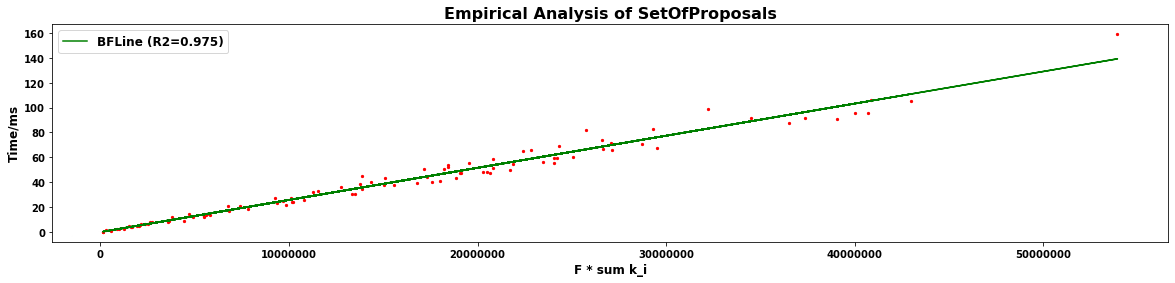
\includegraphics[width = \textwidth]{q6d.png}
\end{figure}
\noindent This plotted graph is based on a data set of 100 samples. We observe a linear relationship between the time taken in \(ms\), and the number  (\(F \times \sum_{i=1}^n k_i\)). The best fit line has a \(R^2\) coefficient of \(0.975\), which means that the linear model fits the data set well. Hence, we could conclude that the time complexity of the algorithm is some constant times \(F \times \sum_{i=1}^n k_i\), and hence there is \(c, n_0 > 0\) such that \(T(n) \leq c(F\times \sum_{i=1}^n k_i)\) for all \(n \geq n_0\). Time complexiy is therefore \(O(F \times \sum_{i=1}^n k_i)\) and the empirical analysis matches with our theoretical analysis. 

\bibliography{citation}

\end{document}